\documentclass{article}
\usepackage[paper=a4paper,margin=2.5cm]{geometry}
\usepackage[utf8x]{inputenc}
\usepackage[francais]{babel}
\usepackage[hidelinks]{hyperref}
\usepackage{listings}
\usepackage{nameref}
\usepackage{graphicx}
\usepackage{xcolor}
\usepackage{tikz}
\usepackage{fix-cm}
\definecolor{noirp8}{cmyk}{0,0,0,0.97}
\definecolor{rougep8}{cmyk}{0,.82,.80,0.18}
\usetikzlibrary{decorations.text}
\usepackage{float}
\usepackage{tikz}
\usetikzlibrary{shapes,shadows,arrows}
\usepackage{harvard}
\usepackage{hyperref}



\author{AHN HARAM}
\title{La production de jeu vidéo avec Pygame avec la théorie de mathématique et la connaissance basique de codage}
\date{\today}

\begin{document}

\begin{titlepage}
  \sffamily
  \noindent
  \begin{minipage}{0.7\linewidth}
    \raggedright
    
\includegraphics[height=2cm]{p8}\\
    \medskip

    \large
    Université Paris 8\\
    Licence informatique \& vidéoludisme\\
    \url{https://informatique.up8.edu/licence-iv/}
  \end{minipage}
  \begin{minipage}{0.3\linewidth}
    \raggedleft
    \resizebox{!}{4cm}{%
      \begin{tikzpicture}
        \draw (0,0) ellipse (152mm and 211mm);
        \draw (0,0) ellipse (144mm and 201mm);
        \clip (0,0) ellipse (144mm and 201mm);
        \fill[noirp8] (-77,0) rectangle (144, 100.5);
        \fill[rougep8] (-77,0) rectangle (144, -100.5);
        \draw[color=white, line width=5pt] (0,0) ellipse (100mm and 160mm);
        \draw[color=white, line width=5pt] (0,0) ellipse (100mm and 160mm);
        \path[postaction={decoration={text along path, text format delimiters={|}{|},
            text={|\sffamily\fontsize{100}{120}\selectfont\color{white}|UNIVERSIT{É} PARIS 8},
            text align=center}, decorate}] (-10,6.5) arc (155:25:110mm and 180mm);
        \path[postaction={decoration={text along path, text format delimiters={|}{|},
            text={|\sffamily\fontsize{95}{114}\selectfont\color{white}|INFORMATIQUE {\&} VID{É}OLUDISME},
            text align=center}, decorate}] (-13.5,-1) arc (180:360:135mm and 180mm);
        \node[color=white] at (0,4) {\sffamily\fontsize{120}{144}\selectfont\color{white}LICENCE};
        \node[color=white] at (0,-5) {\sffamily\fontsize{300}{360}\selectfont\color{white}IV};
      \end{tikzpicture}%
    }
  \end{minipage}

  \vfill

  \begin{center}

    {\Huge \textbf{Pygame rapport}}

    \vfill

    \begin{abstract}
   L'augmentation explosive de la demande de développement de jeux a permis à n'importe qui de créer des jeux. Nous avons créé un jeu à partir de connaissances de base en codage et en théorie simple de la mathématique. Le code utilisé et la théorie mathématique ont mis en œuvre le jeu avec des algorithmes faciles à comprendre
    \end{abstract}

  \end{center}

  \vfill

  \large

  \textbf{Haram \textsc{AHN}}
  \hfill
  numéro étudiant 21000519


  haram.ahn02@etud.univ-paris8.fr
  \hfill
  L1 informatique groupe B

  \url{http://haram3092.dothome.co.kr }
  \hfill
  année universitaire 2021--2022


\end{titlepage}
\maketitle
\clearpage
\tableofcontents
\newpage
\section{Introduction}

\vspace{1cm}
Cela ne fait pas longtemps que le jeu est inclus dans le domaine académique. Le jeu a existé depuis les débuts de la civilisation humaine, Or le jeu n’est pas traité comme un sujet d’étude avant le 20ème siècle. L'origine peut être attribuée à 'Homo Ludens'\footnote{Homo ludens est une expression utilisée pour la première fois par Johan Huizinga dans son ouvrage Homo ludens, essai sur la fonction sociale du jeu} de Johan Huizina\footnote{Johan Huizina: né le 7 décembre 1872 à Groningue et mort le 1er février 1945 à De Steeg, est un historien néerlandais, spécialiste de l’histoire culturelle dans la lignée de Jacob Burckhardt} en 1938. Johan Huizina s’intéresse au jeu comme une étude initialement. Il définit la racine de l’Homme comme le jeu, et dans ce cas, la conception du jeu contient le plaisir moral et la créativité humaine. Il découvrit également que le jeu remonte aux cérémonies du chamanisme de l’époque ancienne. Il contribue à ce que le jeu parvienne à avoir une stature en tant qu’étude légitime.


Le commencement du jeu vidéo électronique est connu comme 'Tennis or Two'. Il crée le jeu pour amuser des visiteurs de laboratoire Brookhaven\footnote{le laboratoire national de Brookhaven ou Brookhaven National Laboratory (BNL) en anglais, est un laboratoire national américain basé à Brookhaven, dans le hameau d'Upton, sur Long Island}, ce jeu est non seulement l’origine de jeu commercial mais inspire aussi le jeu ‘pong’ qui sert à la massification du jeu vidéo électronique. Steve Russell(1962)\footnote{Steve Russell ( Stephen Russel) dit Slug: né en 1937, est informaticien et un des programmeurs à l'origine du jeu 'Spacewar'}  produit le jeu ‘space war’ qui est disponible sur ordinateur, et Ralph Henry Baer\footnote{Ralph Henry Baer: né le 8 mars 1922 à Pirmasens, et mort le 6 décembre 2014 à Manchester aux États-Unis est un inventeur germano-américain.Baer a apporté de nombreuses contributions au domaine du jeu vidéo, notamment la console à usage domestique raccordée à la télévision. Il est parfois surnommé « le père des jeux vidéo ». La National Medal of Technology and Innovation lui est remise en 2006. Il est introduit au National Inventors Hall of Fame en 2010.} fabrique le jeu ‘Odyssey’ qui fonctionne sur télévision. Nolan Bushnell(1972)\footnote{Nolan Bushnell: né le 5 février 1943 à Clearfield dans l'Utah, est un pionnier de l'industrie du jeu vidéo aux États-Unis. Il est le concepteur de Pong et le fondateur d'Atari}, conçu comme le père de jeu vidéo électronique, fonde l’entreprise de jeu vidéo Atari\footnote{Atari est une entreprise française de jeu vidéo, dont le siège est situé à Paris, en France.} et produit le jeu 'Computer Space', 'Pong'. Ses jeux réussissent à populariser le jeu vidéo.


Après que l’industrie du jeu vidéo parvienne à produire d’importants profits commerciaux, les plateformes de jeu indépendantes sont apparues avec la réussite du l’industrie du jeu vidéo. Grâce au développement de plateformes de jeu indépendantes, des personnes appartenant à différents groupes professionnels participent à la fabrication de jeux vidéo. On s'intéresse alors à savoir si n'importe qui peut produire un jeu. Dans ce rapport, nous décrivons qu’il est possible de réaliser le jeu vidéo avec une théorie mathématique simple et un niveau de codage basique. Notre but est de focaliser à réaliser les fonctions fondamentales d’un jeu avec un bas niveau de code.

  
\vspace{1cm}  
\begin{figure}[h]
    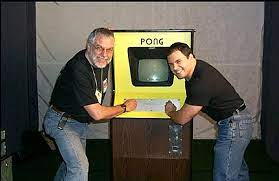
\includegraphics[width=8cm]{image_1.jpeg}\hfill
    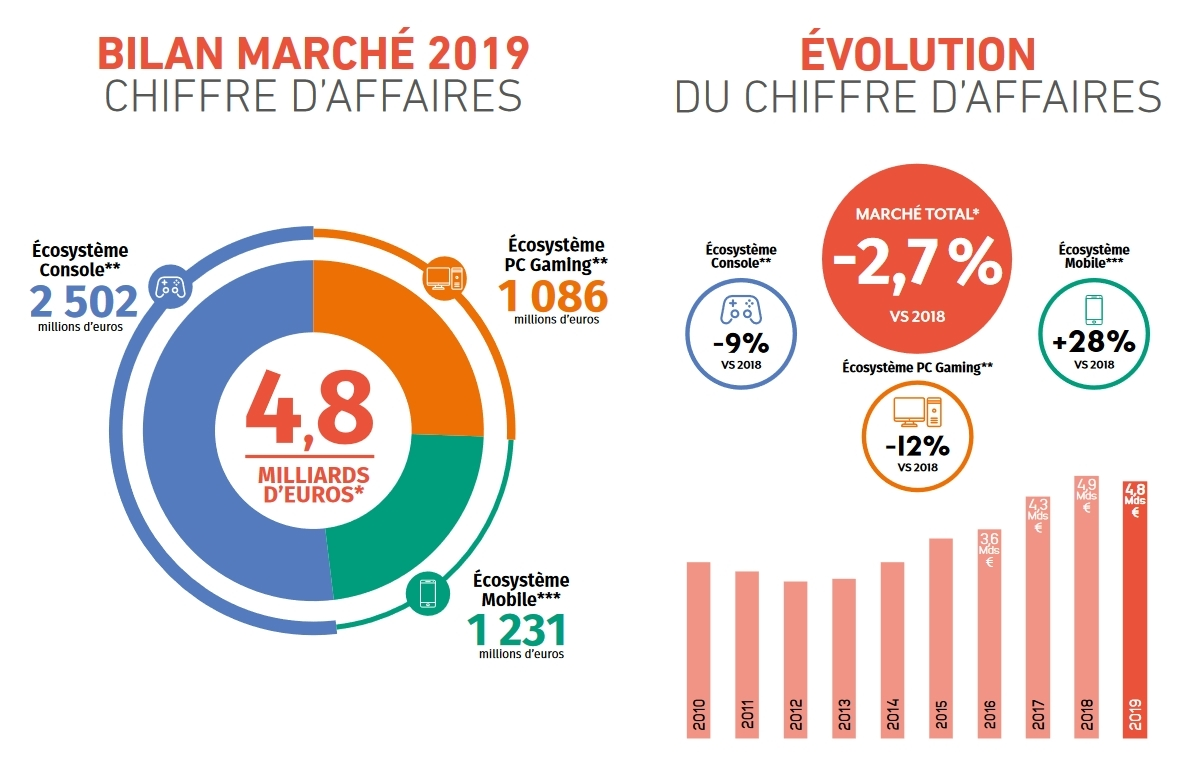
\includegraphics[width=8cm]{l'argmentation.jpeg}
    \caption{le jeu initial  et le marche de jeu vidéo actuelle}
\end{figure}
\newpage
\subsection{scénario}
Pour animer ce projet, on fixe le principal basique


1. logique


- Comme le sujet de ce rapport, notre but est de réaliser le jeu simple avec une connaissance basique de codage, dès lors le jeu à réaliser doit être simple, la logique aussi doit être simple.


2. collusion


- Pour réaliser la collusion entre un hameçon et un poisson, on a besoin de la théorie de la fonction primaire.


3. la fonction utilisée pour réaliser le jeu


Pour accéder aux informations nécessaires à propos de la fonction, nous consultons les sites suivants :


  - \href{https://www.pygame.org/docs/ref/rect.html}{Pygame Tutorial}
  
  
  - \href{https://stackoverflow.com}{Stackoverflow}

\subsubsection{ le processus de production}

\usetikzlibrary{shapes,shadows,arrows}

\tikzstyle{decision} = [diamond,draw,fill=blue!50]
\tikzstyle{line} = [draw,-latex',-stealth,thick]
\tikzstyle{elli} = [draw,ellipse,fill=red!50,minimum height = 5em , node distance = 10em]
\tikzstyle{block} = [draw,rectangle,text centered,fill=blue!50,text width = 8em,minimum height = 15mm,node distance = 10em]

\begin{tikzpicture}
\node[block] (start) {production du jeu vidéo};
\node[block, left of = start, xshift= -5em] (process1) {organisation de l'algorithmiques};
\node[block, above of = start,xshift=-15em, yshift = 5em] (user) {création de ressources};
\node[decision, below of = start,yshift = -10em] (process2){Finalisation du projet};
\node[block, right of = start, xshift = 5em] (process3) {problème technique};
\node[elli, right of = user, xshift = 20em] (process4) {consulter le site de codage};
%arrows
\path[line,thick] (process4) -- (process1);
\path[line,thick] (process1) -- (process4);
\path[line,thick] (user) -- (start);
\path[line,thick] (start) -- (user);
\path[line,thick] (start) -- (process1);
\path[line,thick] (process1) -- (start);
\path[line,thick] (start) -- (process3);
\path[line,thick] (process3) -- (start);
\path[line,thick] (start) -- (process2);
\path[line,thick] (process4) -- (user);
\path[line,thick] (user) -- (process4);
\path[line,thick] (process3) -- (process4);
\path[line,thick] (process4) -- (process3);
\path[line,thick] (start) -- (process4);
\path[line,thick] (process4) -- (start);
\path[line,thick] (user) -- (process1);
\path[line,thick] (process1) -- (user);
\end{tikzpicture}

\subsubsection{le régle général du jeu vidéo à réaliser}
Il y a une limite du temps, il faut cliquer quand l’hameçon qui bouge arrive à l’angle où des poissons se situent. Si des utilisateurs pêchent l’empêchement, ils sont pénalisés. S’ils arrivent au note goal, ils gagnent
\newpage
\section{Algorithme}
\subsubsection{charger des fichiers de l'image}
Tout d’abord, il faut appeler le fichier afin de créer le jeu. Il existe diverses méthodes pour charger le fiche sur Pygame.
\subsubsection{harger l’image du fond}
D’abord, il faut mettre os.path.dirname\verb|(__file__)|  dans current path et créer la valeur background qui enregistre l’adresse de fichier du l’image du fond. On utilise la fonction os.path.join pour retrouver l’adresse du fichier et le nom et appeler l’image avec la fonction pygame.image.load. Ensuite, on charge l’image de background avec la fonction screen.blit. La valeur pour la fonction screen.blit doit être (0,0) et on met à jour avec la fonction pygama.display.update() sur l’écran.\newline

Background = pygame.image.load(os.path.join\verb|current_path|,\verb|”banckgroind_modifi_size.png”))|

\subsubsection{personnage}
Afin de diversifier le moyen de charger le fiche de l’image, on n’a pas utilisé la fonction os.path.join.  Il faut créer la valeur Character et on enregistre l’adresse du fichier par le chemin définitif dans la fonction pygame.image.load(). On utilise la fonction get.rect().size pour calculer la longueur et le hauteur de personnage.\newline

Character = pygame.image.load(os.path.join(\verb|current_path|,"personnage.png"))
\subsubsection{ charger des poissons et des empêchements}
Il est possible de charger des images de poissons et des empêchements de la manière mentionnée dans les parties 2.0.1 et 2.0.2 dans le cas où il y a beaucoup de fiches qui chargent, cette manière est très inefficace et cause des difficultés pour gérer les fichiers. Afin de résoudre ces problèmes, on crée une liste afin de les gérer facilement et on ajoute une méthode utilisée pour enregistrer des valeurs de des hauteurs et des longueurs des fichiers. Il faut hériter Sprite offrit par le Python dans notre algorithme. Cependant, il est indépendant de créer une classe pour hériter Sprite, et on utilise aussi \verb|super._init()| pour la valeur initiale. Il est obligé de créer des variable membre pour user cette fonction pour cela, on crée une valeur de self.image dans la classe et on utilise la fonction get.rect() pour stocker les informations de la position. On fixe que la valeur de center est égale à la valeur de la position.


On utilise une méthode pygame.sprite.Group() à la façon de créer un group des informations stocké dans une liste \verb|image_group|, on gère les informations par une méthode \verb|setup_poisson()|. On ajoute les fichier suplémentaire avec la formule tuple et après on use la fonction de add.\newline

\verb|def setup_possion()|:


\verb|small_poisson = (Poisson(les_images[0]|,(400,700),possion\verb|_petit_price,poisson|


\verb|_petit_vitesse))|
   \verb|image_group.add(small_poisson)|\newline

Cependant il faut créer deux lignes inutiles, on choisit d’ajouter le fichier dans la liste \verb|Image_group| avec la fonction add directement.
 
 
 \verb|def setup_possion():|

\verb|image_group.add(Poisson(les_images[0],| (400,700),\verb|possion_petit_price,poisson_petit_|

vitesse))
\subsubsection{la création de hameçon et de cordeau}
On charge le fichier de l’image de l’hameçon par la même méthode avec 2-2 nous définissons une classe dans notre algorithme pour donner la fonction supplémentaire. On donne la valeur de position (1100,420), cette valeur est identique avec les coordonnées d'une fonction primaire. 


Quand on essaie à mettre à jour en utilisant la fonction de draw, on rencontre le message de l’erreur, car chaque sprite ne offert pas la fonction de draw. Pour résoudre ce problème, on définit une méthode dans la classe de Galgori. Un hameçon doit bouger d'un côté à l’autre, pour cela il faut charger l’image de hameçon dans la position un peu loin du point de centre, alors on définit le constant valeur 40 nommé default\verb|_offset_x_galgori| avec le formulaire int et mettre à jour par la fonction pygame.math.Vector2. Afin de fabriquer un cordeau on utilise la fonction draw.line() offrit Python.\newline

 self.offset = pygame.math.Vector2(\verb|default_offset_x_galgori|,0)
\subsubsection{ Le mouvement de hameçon}
d’expliquer d’abord, une gamme de mouvements. On fixe 175° pour la gamme maximale de mouvement d’hameçon et 10° pour la gamme initiale de mouvement de hameçon. Afin de réaliser le mouvement, on ajoute une code qui additionne ou soustraite le valeur nommé \verb|self.angle_speed| contenant le valeur int 2.5 au gamme initiale de mouvement de hameçon dans une méthode \verb|def __init__()| et on ajoute une méthode def update() pour calculer la gamme de mouvement.\newline

\begin{tikzpicture}
  \draw[->,thick] (-3,0) -- (3,0);
  \draw[->,thick] (0,-3) -- node[below=3cm]{la gamme de mouvement} (0,3);
  \draw[very thick,red] (0,0) -- node[left]{$175^\circ$} (-1.5,-1.5);
  \draw[very thick,red] (0,0) -- node[right]{$10^\circ$} (1,-1.5);
\end{tikzpicture}
\vspace{1cm}


\verb|def __init__|(self, image, position):


\verb|super().__init__()|:

self.image = image


self.rect = image.get.rect(center = position)


\verb|self.original_image =image|


self.direction = LEFT


\verb|self.angle_speed| = 2.5


self.angle = 10


self. direction = LEFT


\verb|self.angle_speed|\newline

def update(self):


if self.direction == LEFT:
\verb|self.angle += self.angle_speed|


elif self.direction == RIGHT:


\verb|self.angle -= self.angle_speed|

\vspace{1cm}
De sorte de réaliser les caractéristiques d’animation avec le code qui calcule la gamme de mouvement du hameçon, on ajoute la fonction pygame.transform.rotaezoom dans une méthode nommé rotate() . Or, on estime l’image qui bouge hors de la gomme fixé afin de régler ce problème, on refixe la gamme de mouvement par self.position.\newline

def rotate(self):

self.image = pygame.transform.rotaezoom\verb|(self.original_image,- self.angle, 1)|


self.rect = self.image.\verb|get_rect(center = self.position + offset_rotated)|
\subsubsection{Collusion des images}
Pour réaliser la collusion entre un hameçon et les poissons, on programme que le poisson est éliminé dans une liste nommé \verb|image_group| si un hameçon atteint les valeurs de coordonnées des poissons. Cependant, il est impossible de réaliser l’animation de pêche réellement, pour cela on utilise la théorie mathématique basique, plus exactement, la fonction trigonométrique.

\subsubsection{démonstraction mathématique}


On convert le valeur de seta vers le radians.


\vspace{1cm}
\begin{tikzpicture}
  \draw[->,thick] node[left=1.5cm,above,red]{$180^\circ$}(-3,0) --node[right=1.7cm,above,red]{$0^\circ$} (3,0);
  \draw[->,thick] node[above=1.7cm,right,red]{$90^\circ$}(0,-3) -- node[below=1.7cm,right,red]{$270^\circ$} (0,3);
  \draw[thick] (0,0) circle[radius=2];
\end{tikzpicture}
\vspace{3cm}
\begin{tikzpicture}
  \draw[->,thick] node[left=1.7cm,above,red]{$\pi$}(-3,0) -- node[right=1.7cm,above,red]{$0\pi$} (3,0);
  \draw[->,thick] node[above=1.7cm,right,red]{$\frac{1}{2}\pi$}(0,-3) -- node[below=1.7cm,right,red]{$\frac{3}{2}\pi$}(0,3);
  \draw[thick] (0,0) circle[radius=2];
\end{tikzpicture}\newline

import math


print(“radians \verb|0°:|”

,math.radians(0),”\verb|\nradians 90°:”,math.radians(90),”\nradians 180°:”,math.radians(180),”|

\verb|\nradians 270°:”,math.radians(270))|


Returne:

radians 0°: 0.0 


radians 90°: 1.5707963267948966 


radians 180°: 3.141592653589793 


radians 270°: 4.71238898038469\newline


\begin{tikzpicture}

  \draw[->,thick] (-3,0) -- (3,0);
  \draw[->,thick] (0,-3) -- (0,3);
  \draw[thick] (0,0) circle[radius=2];
  
  \draw[thick] (0,0) -- (60:2);
  \draw[very thick,blue] (0,0) -- node[below]{$\cos(\theta)$}(1,0);
  \draw[very thick,red] (1,0) -- node[right] {$\sin(\theta)$} (1,2*sin{60});
  
  \filldraw[draw=green,fill=green!30] (0.5,0) arc[radius=0.5,start angle=0,end angle=60] node[below=0cm]{$\theta$} -- (0,0) -- cycle;
  
\end{tikzpicture}

\vspace{1cm}
Soit r est égale à 1\newline

$\sin\theta = \frac{y}{r}$


Alors on peut dire $\sin\theta = y$


$\cos\theta = \frac{x}{r}$


Alors on peut dire 

$\cos\theta = x$


Par conséquent, grâce au principe de la fonction triangulaire, nous pouvons obtenir les coordonnées
\subsubsection{convertir vers le code}
$\sin\theta = \frac{y}{r}$


$\cos\theta = \frac{x}{r}$


On peut simplifier cette formule.


$r\times\sin\theta = y$


$r\times\cos\theta = x$

On peut convertir cette formule comme le code suivant dans son algorithme:


import math
 
 
r = self.rect.size[0] // 2 \verb|\#pie|
  

\verb|rad_angle| = math.radians(angle) \verb|#angle|


x = r * math.cos\verb|(rad_angle)|


y = r * math.sin\verb|(rad_angle)|
\subsubsection{La formule de calcul sous la condition que la collusion arrive}
\begin{tikzpicture}
\draw[->,thick](-1,0) -- (4,0); 
\draw[->,thick](0,-1) -- (0,3); 
\draw[thick] (0.15,0.15) -- (45:2);
\draw[thick] (0.15,0.15) -- node[below]{$\cos(\theta)$}(1.42,0.18);
\draw[thick,red] (0.15,0.18) -- (0.15,0.15);
\draw[very thick] (1.42,0.18) -- node[right] {$\sin(\theta)$} (1.42,2*sin{45});
\draw[thick,green] node[above=1cm,left]{un hameçon} (0.5,0.5) circle[radius=0.5];
\draw[thick,red] node[above=2cm,right=2cm]{un poisson}(1.42,1.42) circle[radius=0.8];
\end{tikzpicture}
\vspace{1cm}


Soit $r’+r = L$


$\sin\theta = \frac{y}{L}$


$\cos\theta = \frac{x}{L}$


On peut dire


$L\times\sin\theta = y$


$L\times\cos\theta = x$


Alors on peut convertir vers code:


self.rect.center = ( position[0] + x, position[1] + y)
\newpage

\section{conclusion}
Nous avons réussi à réaliser un jeu simple avec une logique et une théorie simple de mathématique. Contrairement au plan initial, il y avait des parties difficiles à mettre en œuvre avec des théories mathématiques très élémentaires, mais le jeu a été réalisé au niveau mathématique du lycée. Il n’est pas difficile de réaliser un jeu avec une compréhension mathématique de niveau lycéen et des connaissances basiques de codage. 


Or, du fait que la technique de production de jeu vidéo électronique, des performances informatiques progressent de jour en jour, ainsi de nouvelles plateformes sont apparues comme les smartphones, et alors les capacités demandées aux développeurs de jeu vidéo deviennent élevées. En plus, Pour satisfaire aux demandes variées des consommateurs sur le marché du jeu vidéo, le processus de la production de jeu vidéo devient sophistiqué et subdivisé.  En conclusion, le niveau plus élevé de codage sera demandé afin de réaliser un jeu actuellement. 
\end{document}
